\documentclass[11pt]{amsart}

\usepackage[utf8]{inputenc}
\usepackage{amsmath,amssymb,amsthm,mathtools}
\usepackage[margin=1.1in]{geometry}
\usepackage{graphicx}
\usepackage{booktabs,array}
\usepackage{tikz}
\usetikzlibrary{arrows.meta,positioning}
\usepackage[hidelinks,pdftitle={Euler's Identity, Elliptic Curves and an AI Laboratory},pdfauthor={H. P. Alesso}]{hyperref}
\usepackage{xcolor}
\usepackage{microtype}

\numberwithin{equation}{section}
\newtheorem{hypothesis}{Hypothesis}

\newcommand{\Q}{\mathbb{Q}}
\newcommand{\R}{\mathbb{R}}
\newcommand{\C}{\mathbb{C}}
\newcommand{\Z}{\mathbb{Z}}
\newcommand{\Gal}{\operatorname{Gal}}
\newcommand{\GL}{\mathrm{GL}}
\newcommand{\SL}{\mathrm{SL}}
\newcommand{\Br}{\operatorname{Br}}
\newcommand{\sgn}{\operatorname{sgn}}
\newcommand{\cyc}{\mathrm{cyc}}
\newcommand{\Kfield}{\Q(\sqrt{5})}

\begin{document}

\title{Euler's Identity, Elliptic Curves and an AI Laboratory}

\author{H. P. Alesso}
\address{AI HIVE}
\email{alesso@alum.mit.edu}

\date{October 2026}

\begin{abstract}
Euler's identity $e^{i\pi}=-1$ can be read as a half turn around the circle: it singles out $-1$, the only number other than $1$ whose square is $1$, a switch with two positions. Number theory attaches such plus-or-minus signs to many of its objects, and they often decide something important, such as whether an equation has finitely or infinitely many rational solutions. We argue that a great many of these signs share one source, the contribution of the real numbers (the ``real place''), and we trace it through the Langlands program, from the root number of every elliptic curve over $\Q$ to the quaternions, the real Weil group and the oddness of modular Galois representations, ending with eight research directions. We then describe Artemis, an open-source laboratory in which AI agents run pre-registered computational experiments that a frozen, fingerprinted program judges, and report its first test. Over $\Kfield$, which has two real places, so that the two half turns cancel, murmurations of elliptic curves follow $+\prod_{\mathfrak p}w_{\mathfrak p}$, the reverse of the rule over $\Q$, as theory predicts (correlation $0.53$, 95\% interval $[0.46,0.59]$), although the two patterns part company for large primes. Among curves over $\Q$ with the same conductor, the local signs of rank-$2$ curves differ slightly but certainly from those of rank-$0$ curves: on about $210{,}000$ curves held out until the end, a rule fixed in advance tells the two ranks apart $52\%$ of the time and the laboratory's rule $54\%$ of the time, against $50\%$ for chance ($z=8.6$ and $15.1$). The signal lies chiefly in the size of the bad prime. The final test was reproduced exactly, and all code and data are public.
\end{abstract}

\maketitle

% ======================================================================
\section{Introduction}\label{sec:intro}

Euler's identity, $e^{i\pi}=-1$, is often called the most beautiful equation in mathematics. One way to picture it is as a turn around a circle: start at the number $1$, walk halfway around the circle of radius one, and you arrive at $-1$. In the language of the exponential map $x\mapsto e^{2\pi i x}$, the midpoint $1/2$ of the unit interval goes to $-1$, the unique element of order two on the circle. Minus one is special because it is the only number other than $1$ whose square is $1$; it is a switch with two positions, plus and minus. Three basic facts share this shape: the real numbers contain only the roots of unity $\pm1$; by the Artin--Schreier theorem every nontrivial torsion element of $\Gal(\overline{\Q}/\Q)$ is conjugate to complex conjugation \cite{ArtinSchreier1927}; and $\Br(\R)=\Z/2$, generated by the quaternions, so that the real Weil group is a non-split extension with $j^2=-1$.

Modern number theory is full of such switches. Mathematicians attach a sign, plus or minus, to many of the objects they study, and these signs often decide something important, such as whether an equation has finitely or infinitely many solutions in fractions. Our thesis is that a great many of them share one source. They can be traced to Euler's half turn, which enters whenever the ordinary real numbers, the numbers on a ruler, take part in a calculation; number theorists call this the contribution of the \emph{real place}, as opposed to the contributions of the individual primes $2,3,5,7,\dots$. In the vocabulary of the Langlands program, the signs of the program are incarnations of this one $\Z/2$, and Euler's identity is the formula that places the sign inside analysis. On the Galois side the sign is the value $\chi_\cyc(c)=-1$ of the cyclotomic character on complex conjugation; on the automorphic side it is $\psi_\infty(1/2)=-1$ for the standard additive character, and $i^2=-1$ is the archimedean root number of every elliptic curve over $\Q$ \cite{Deligne1973}. Its most compact form is Tate's local constant at the real place, $\varepsilon(s,\sgn,\psi)=i$ \cite{Tate1950}, for which the general relation $\varepsilon(s,\chi,\psi)\varepsilon(1-s,\chi^{-1},\psi)=\chi(-1)$ reads
\begin{equation}\label{eq:thesis}
i\cdot i=\sgn(-1)=-1 .
\end{equation}

The paper has three parts. Section~\ref{sec:synthesis} is a guided tour of where this one minus sign turns up across the program. Nothing there is new mathematics; the aim is to organize known results around one element of order two and to draw questions from the organization. A reader interested mainly in the experiment can skim it: what matters later is that every elliptic curve over $\Q$ carries a sign built from one small sign per bad prime and one extra $-1$ from the real place. Section~\ref{sec:artemis} describes Artemis, an autonomous laboratory that we built to test such questions by computation, and Sections~\ref{sec:experiment} and~\ref{sec:discussion} report and discuss its first run, a test of research direction R1 on elliptic curves. Section~\ref{sec:directions} states eight research directions. Statements marked [T] are theorems in the literature, [C] conjectures, [O] open questions and [P] proposals that can be tested by computation now.

% ======================================================================
\section{The archimedean sign across the program}\label{sec:synthesis}

Table~\ref{tab:map} summarizes where the sign appears; the paragraphs below give the main points with references.

\begin{table}[ht]
\centering\small
\caption{One element of order two, seen from different parts of the program.}\label{tab:map}
\begin{tabular}{@{}>{\raggedright\arraybackslash}p{0.27\textwidth}>{\raggedright\arraybackslash}p{0.33\textwidth}>{\raggedright\arraybackslash}p{0.32\textwidth}@{}}
\toprule
Setting & Form of the sign & Meaning\\
\midrule
Fourier analysis, Tate's thesis & $\psi_\infty(1/2)=-1$; $\varepsilon(\sgn)=i$ & Euler factor and local constant at $\infty$\\
$\GL_1$, reciprocity & Gauss sum signs; Weil index $e^{i\pi/4}$ & Quadratic reciprocity as a product formula\\
Real Weil group, Hodge theory & $j^2=-1$; Weil operator $C$ with $C^2=(-1)^w$ & Parameters at $\infty$ are Hodge structures\\
$\GL_2$, elliptic curves & $i^k$; $w(E)=-\prod_{p\mid N}w_p$; $\det\rho(c)=-1$ & Parity of rank; oddness; Heegner points\\
Endoscopy, classical groups & Component groups are $2$-groups; Kottwitz sign & Arthur's sign characters\\
Periods & $2\pi i$, period of $\Q(1)$ & Deligne's conjecture; $\zeta(2k)\in\Q\,\pi^{2k}$\\
$p$-adic, function fields & Dwork's $\pi$; Fontaine's $t$; Carlitz's $\tilde\pi$ & Analogues of $2\pi i$\\
Sato--Tate, murmurations & CM Sato--Tate group; $a_p$ correlated with $w(E)$ & Equidistribution; Zubrilina's theorem\\
\bottomrule
\end{tabular}
\end{table}

\emph{Euler's two formulas.} An L-function joins Euler's product over primes to Euler's exponential at the infinite place. The finite Euler factors are periodic in $s$ because $e^{2\pi i}=1$, and the archimedean factor is the Gamma function $\pi^{-s/2}\Gamma(s/2)$ because the Gaussian $e^{-\pi x^2}$ is its own Fourier transform for the kernel $e^{-2\pi i x\xi}$ \cite{Tate1950}. Langlands' program asserts that every Euler product from arithmetic is automorphic \cite{LanglandsProblems1970}.

\emph{Fourier analysis and the Weil representation.} With the kernel $e^{-2\pi i x\xi}$ the square of the Fourier transform is the parity operator $f(x)\mapsto f(-x)$, which acts by $e^{i\pi}=-1$ on odd functions. In the Weil representation the element $S=\left(\begin{smallmatrix}0&-1\\1&0\end{smallmatrix}\right)$ acts as the Fourier transform up to an eighth root of unity, and $S^2=-I$ acts on forms of weight $k$ by $(-1)^k$; this is why there are no nonzero modular forms of odd weight for $\SL_2(\Z)$, and why half-integral weight needs a double cover [T]. More generally, local root numbers of a self-dual representation square to the value of its central character at $-1$, so they are fourth roots of unity whose square is decided by Euler's $-1$ \cite{Tate1979}.

\emph{$\GL_1$ and reciprocity.} Class field theory over $\Q$ is generated by values of Euler's exponential at rational points, and Euler's criterion $g^{(p-1)/2}=-1$ is the finite-field form of the identity. The sign of the quadratic Gauss sum, $g_p=\sqrt p$ or $i\sqrt p$, which Gauss determined in 1805, is the first root number in history; it depends on the embedding of $e^{2\pi i/p}$ into $\C$ \cite{Gauss1811}. Weil showed that the real place contributes the eighth root of unity $\int_\R e^{i\pi x^2}dx=e^{i\pi/4}$ to a product formula whose truth is quadratic reciprocity \cite{Weil1964}; the real invariant of the quaternions in the Brauer group is $1/2$, which Euler's exponential turns into $-1$ [T].

\emph{The real Weil group.} Local Langlands parameters at the real place are homomorphisms from $W_\R=\C^\times\sqcup j\C^\times$ with $j^2=-1$ \cite{Langlands1973}. For a motive of weight $w$, the image of $-1$ is $(-1)^w$, and the restriction of the parameter to $\C^\times$ is the Hodge structure, whose Weil operator $C$ satisfies $C^2=(-1)^w$; the Tate motive $\Q(1)$ is odd because complex conjugation acts on its period $2\pi i$ by $-1$ [T]. Kottwitz's sign of a real group \cite{Kottwitz1983} is the same $-1$ for the quaternions.

\emph{$\GL_2$ and the parity of rank.} The tour becomes testable through elliptic curves, equations such as $y^2=x^3-x+1$. A central question about such a curve is how many solutions it has in fractions: some have only a handful, others infinitely many, generated from a few basic solutions, and the number of independent basic solutions is the \emph{rank}. Every curve also carries a sign, its root number $w(E)$, which is predicted to tell whether the rank is even or odd. That sign is assembled from one small sign $w_p$ for each bad prime $p$, where the equation breaks down modulo $p$, and from one extra factor contributed by the real place. For a modular form of weight $k$ that archimedean factor is $i^k$; for elliptic curves ($k=2$) it is $i^2=-1$, Euler's half turn, so
\begin{equation}\label{eq:rootQ}
w(E)=-\prod_{p\mid N}w_p(E)
\end{equation}
[T]. The Birch--Swinnerton-Dyer conjecture predicts $(-1)^{\mathrm{rank}}=w(E)$, and the $p$-parity conjecture is a theorem over $\Q$ \cite{DokchitserDokchitser2010}. Over a totally real field of degree $d$ there are $d$ real places, hence $d$ half turns, and the archimedean factor becomes $(-1)^d$. The same sign makes every modular Galois representation odd, $\det\rho(c)=-1$, and odd representations are exactly those covered by Serre's conjecture \cite{KhareWintenberger2009}; the even side remains largely open \cite{Calegari2011}. Heegner points exist because imaginary quadratic characters are odd: when every prime dividing $N$ splits in $K$, this forces the root number of $E$ over $K$ to be $-1$ \cite{GrossZagier1986}.

\emph{Sato--Tate and murmurations.} The Sato--Tate group of a CM elliptic curve is, as a compact group, the maximal compact subgroup of $W_\R$, and Frobenius at inert primes lies in its $j$-component, where the trace vanishes [T]. Count the solutions of a curve modulo a prime $p$, as on a clock face; the deviation from $p+1$ is the number $a_p$. He, Lee, Oliver and Pozdnyakov, with the help of machine learning, observed that the averages of $a_p$ over many curves in a conductor range rise and fall in a wave as $p$ grows, like the shifting shape of a flock of starlings \cite{HLOP2022}; Zubrilina proved that for modular forms the leading term of this ``murmuration'' is a correlation between $a_p$ and the root number \cite{Zubrilina2023}, and the same is expected for elliptic curves ordered by conductor [C]. The split by rank parity in every murmuration plot is therefore a split by \eqref{eq:rootQ}, archimedean sign included.

\emph{The general program.} The component groups that organize L-packets of classical groups are elementary abelian $2$-groups, so the structure of a packet is a matter of signs \cite{Arthur2013}. Deligne showed that local constants of orthogonal representations are governed by a second Stiefel--Whitney class \cite{Deligne1976}, and the corresponding global product formula, like those of Hilbert and Kottwitz, is a statement about $2$-torsion in the Brauer group with a term at the real place. Poonen and Stoll's criterion for the order of the Tate--Shafarevich group of a Jacobian to be twice a square \cite{PoonenStoll1999} is another product formula of local signs with an archimedean term, and Bella\"iche and Chenevier proved that the polarizations of Galois representations attached to conjugate-self-dual automorphic representations over CM fields always carry the expected sign \cite{BellaicheChenevier2011}. In geometric Langlands and its physical interpretation \cite{KapustinWitten2007}, the choice of a square root of the canonical bundle, the spin double cover and the $\theta$-angle $\pi$ all carry the same $\Z/2$.

\emph{Periods.} $2\pi i$ is the period of the Tate motive, and $\zeta(2k)=-\frac{B_{2k}}{2(2k)!}(2\pi i)^{2k}$ is the case of Deligne's period conjecture \cite{Deligne1979} for $\Q(0)$; the minus sign in $\zeta(2)=-(2\pi i)^2/24$ is $i^2$. Because the only units of $\Z$ are $\pm1$, the Tate motive has no nontrivial extensions over $\Z$, which underlies the structure of mixed Tate motives over $\Z$ \cite{DeligneGoncharov2005,Brown2012}.

\emph{Other analogues.} Dwork's $\pi$ with $\pi^{p-1}=-p$ \cite{Dwork1960}, Fontaine's $t$ \cite{Fontaine1994} and Carlitz's period $\tilde\pi$ \cite{Carlitz1935} play the role of $2\pi i$ at $p$ and in function fields. Finally, metaplectic covers of order $n$ require $n$-th roots of unity, so over $\Q$ only the double cover exists; for $n\ge3$ all archimedean places are complex, the Weil index is trivial there, and cubic Gauss sums have no closed-form sign \cite{HeathBrownPatterson1979,DunnRadziwill2024}. Euler's identity is an $n=2$ phenomenon.

Table~\ref{tab:master} collects the incarnations in compact form. Three of Euler's legacies close the circle: his identity, his product, and the Euler characteristic of Galois cohomology, which Tate's formula expresses through the invariants of complex conjugation, the very element whose image under the cyclotomic character is $e^{i\pi}$.

\begin{table}[ht]
\centering\small
\caption{The same $\Z/2$ in different settings.}\label{tab:master}
\begin{tabular}{@{}lll@{}}
\toprule
Object & The $\Z/2$ & Euler form\\
\midrule
Roots of unity in $\R$ & $\{\pm1\}$ & $e^{i\pi}=-1$\\
Torsion in $G_\Q$ & complex conjugation $c$ & $\chi_\cyc(c)=-1$\\
Brauer group of $\R$ & quaternions & $e^{2\pi i\cdot\frac12}=-1$\\
Real Weil group & $j^2=-1$ & $\varphi(j)^2=(-1)^w$\\
Local constants at $\infty$ & $\varepsilon(\sgn)=i$ & $\varepsilon(\sgn)^2=\sgn(-1)$\\
Modular forms & weight parity & $\varepsilon_\infty=i^k$\\
Galois representations & $\det\rho(c)$ & odd means $-1$\\
Component groups & $(\Z/2)^k$ & Arthur's signs\\
Periods & $(2\pi i)^n$ & $\zeta(2k)\in\Q\,(2\pi i)^{2k}$\\
\bottomrule
\end{tabular}
\end{table}

% ======================================================================
\section{Artemis: an autonomous laboratory}\label{sec:artemis}

Several questions raised by the synthesis can be tested on public data. AI agents can now write and run such computations on their own, but an agent that chooses its analyses, sees its results and keeps trying will find patterns that are not there. Artemis (\url{https://github.com/alessoh/artemis}) gives a team of agents wide freedom to propose and test ideas and no freedom over how they are judged. One agent searches the literature, one proposes ideas, several write and test experiments in parallel, a skeptic tries to knock down every apparent success, and a scribe writes the report. A frozen program, whose code and data are sealed with digital fingerprints, scores every experiment; the rules and hypotheses are published before the run; and a final set of data is locked away and used exactly once, at the very end.

\emph{Design.} Two ideas shaped it. The first is a first-principles engineering procedure, described by Isaacson as Elon Musk's ``algorithm'' \cite{Isaacson2023}: question each requirement, delete what can be deleted, simplify, accelerate, and automate last. For a laboratory the requirement that survives is a measurement fixed in advance that the experimenter cannot change; almost everything else was deleted. The second is Karpathy's AutoResearch pattern \cite{Karpathy2026}: an immutable harness holding the data and the metric, a single file the agent edits, and an instruction file written by the human. Artemis keeps these three files, as \texttt{harness.py}, \texttt{experiment.py} and \texttt{program.md}.

\emph{Architecture.} Figure~\ref{fig:architecture} shows the parts. The agents run in Omnigent \cite{Omnigent} inside a cloud sandbox. A lead agent runs the loop and is the only one allowed to promote a trial or run the final test. It directs a Scout that searches the literature with cited sources, a Planner that proposes ideas with stated hypotheses, parallel Experimenters that each implement one idea, a Skeptic that tries to break every candidate before it is kept, and a Scribe that writes the report from the result files. In the run reported here the Scout used Claude Haiku~4.5 and the others Claude Opus~5.5.

\begin{figure}[ht]
\centering
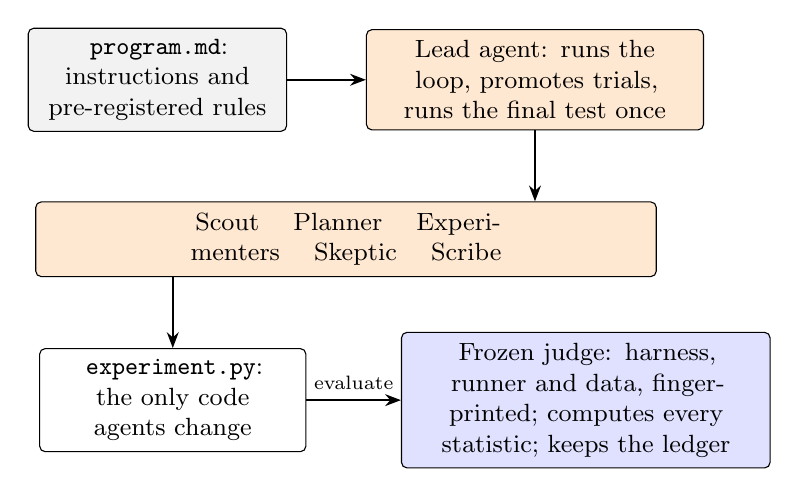
\begin{tikzpicture}[font=\small,
  box/.style={draw, rounded corners=2pt, align=center, minimum height=8mm, inner sep=4pt},
  agent/.style={box, fill=orange!18}, frozen/.style={box, fill=blue!12},
  arr/.style={-{Stealth[length=2mm]}, thick}]
\node[box, fill=gray!10, text width=3.0cm] (prog) {\texttt{program.md}: instructions and pre-registered rules};
\node[agent, right=1.0cm of prog, text width=4.0cm] (lead) {Lead agent: runs the loop, promotes trials, runs the final test once};
\node[agent, below=0.9cm of lead, xshift=-2.4cm, text width=7.6cm] (team) {Scout \quad Planner \quad Experimenters \quad Skeptic \quad Scribe};
\node[box, below=0.9cm of team, xshift=-2.2cm, text width=3.1cm] (trial) {\texttt{experiment.py}: the only code agents change};
\node[frozen, right=1.2cm of trial, text width=4.4cm] (judge) {Frozen judge: harness, runner and data, fingerprinted; computes every statistic; keeps the ledger};
\draw[arr] (prog) -- (lead); \draw[arr] (lead) -- (team.north -| lead); \draw[arr] (team.south -| trial) -- (trial);
\draw[arr] (trial) -- node[above, font=\scriptsize]{evaluate} (judge);
\end{tikzpicture}
\caption{An Artemis program. Agents (orange) can change only the experiment file; the judge (blue) is frozen and fingerprinted.}\label{fig:architecture}
\end{figure}

\emph{The judge.} Every evaluation runs the experiment's single function in a separate process, from a copy of the exact bytes that the harness has just checked, hashed and archived. A static check refuses code that imports anything outside an allowlist, reaches files or the interpreter, or carries large tables of constants, and a run-time hook blocks file access, processes and networking. The experiment sees only what the question allows, and the harness computes every statistic. Budgets count evaluations when they start; a trial is kept only if it beats the current best by a pre-registered margin and survives the Skeptic's review; and the held-out test can run exactly once. Every output carries the fingerprints of the code and data.

\emph{An audit before the run.} A separate agent that had not written the code was asked to attack it. It found that Cremona's tables list the isogeny classes of a conductor in an order correlated with rank: on training data alone, position within the conductor separated rank $2$ from rank $0$ with AUC $0.564$, far more than the signal studied here. The harness now hands each distinct pair of conductor and sign pattern to the experiment once, in sorted order, which removes the leak and makes every result reproducible. The audit also closed several ways around the static check. An agent that noticed this could have scored well without learning any mathematics. We report it because it is a general hazard for anyone who uses AI on curated scientific data: the order and labels of such tables can encode the very quantity under study.

\emph{What protects a result.} The labels in such a program are public mathematics, so integrity cannot rest on secrecy. It rests instead on four things: the experiment sees only what the question allows; the exact code of every trial is archived with its scores; every command of every agent is recorded in the session transcript; and the final test is re-run independently on the promoted code.

% ======================================================================
\section{The experiment and its results}\label{sec:experiment}

Research direction R1 asks two questions. By \eqref{eq:rootQ} the archimedean $-1$ is invisible over $\Q$ because it is always there. It becomes visible when the number system changes. Over $\Kfield$, the numbers built from the square root of $5$, there are two real places, hence two half turns, and minus one times minus one is plus one: the global sign is $+\prod_{\mathfrak p}w_{\mathfrak p}$. Since murmurations follow the global sign, over $\Kfield$ they should line up with the product of the small signs rather than with its opposite, as they do over $\Q$ (Part~A). The second question is new. Curves of rank~$0$ and rank~$2$ over $\Q$ have the same global sign, because both ranks are even; do their small signs, prime by prime, still differ in a systematic way, or is all the difference between them hidden elsewhere (Part~B)?

\emph{Data.} Over $\Q$ we used Cremona's tables \cite{Ecdata} at a pinned commit: every isogeny class with conductor $N<500{,}000$ (of which $790{,}258$ have rank~$0$ and $279{,}056$ rank~$2$), with local root numbers at the bad primes, and $a_p$ computed with PARI/GP \cite{PARI} for the $17{,}314$ classes with $N<5{,}000$. Over $\Kfield$ we used the LMFDB's $4{,}605$ isogeny classes with conductor norm below $5{,}000$ \cite{LMFDB}. Since these curves are modular \cite{FreitasLeHungSiksek2015}, PARI's root number is the sign of the functional equation; we checked that it equals $+\prod_{\mathfrak p}(-a_{\mathfrak p})$ for all $3{,}333$ semistable classes and $(-1)^{\mathrm{rank}}$ wherever the rank is known. The data are frozen and fingerprinted.

\emph{Pre-registration.} All definitions, splits and hypotheses below were committed to the public repository before the run. While building the harness we looked at the training conductors, the pilot ranges of Part~A and the validation score of the simple rule; no one scored the test conductors before the final run.

\subsection{Part A: murmurations over \texorpdfstring{$\Kfield$}{Q(sqrt 5)}}
For each class with conductor (norm) $N$ and each good degree-one prime of norm $p\le N$ we bin $x=p/N$ into ten bins. Over $\Q$ (conductors $1{,}000$ to $4{,}999$), $M_\Q$ is the binned mean of $w\,a_p/\sqrt p$. Over $\Kfield$ (norms $1{,}000$ to $4{,}999$), $F_{ss}$ is the binned mean of $S\,a_{\mathfrak p}/\sqrt p$ over semistable classes, where $S$ is the product of the finite local signs computed from the bad primes alone. The pre-registered statistic is the correlation $\rho_{ss}$ of $F_{ss}$ with $M_\Q$; the prediction is $\rho_{ss}>0$, while carrying over the rule of $\Q$ would give $\rho_{ss}<0$. Intervals come from $2{,}000$ bootstrap draws over conductors.

Over $\Q$ the profiles for $w=+1$ and $w=-1$ are mirror images (correlation $-0.98$), reproducing the published pattern. Over $\Kfield$, $\rho_{ss}=0.5313$ with 95\% interval $[0.4605,0.5944]$: the verdict is consistent with the predicted flip, and it survives using all $3{,}973$ classes with PARI's root number ($0.519$) or dropping base changes from $\Q$ ($0.527$). Figure~\ref{fig:murm} and Table~\ref{tab:partA} show the profiles. The result was expected from Deligne's formula and the parity checks above, so its value is as an explicit demonstration of the archimedean factor inside the murmuration pattern. The agreement is partial: the profiles broadly agree for $x<0.6$, but from $x=0.7$ on the profile over $\Q$ is negative while the one over $\Kfield$ stays positive.

\begin{figure}[ht]
\centering
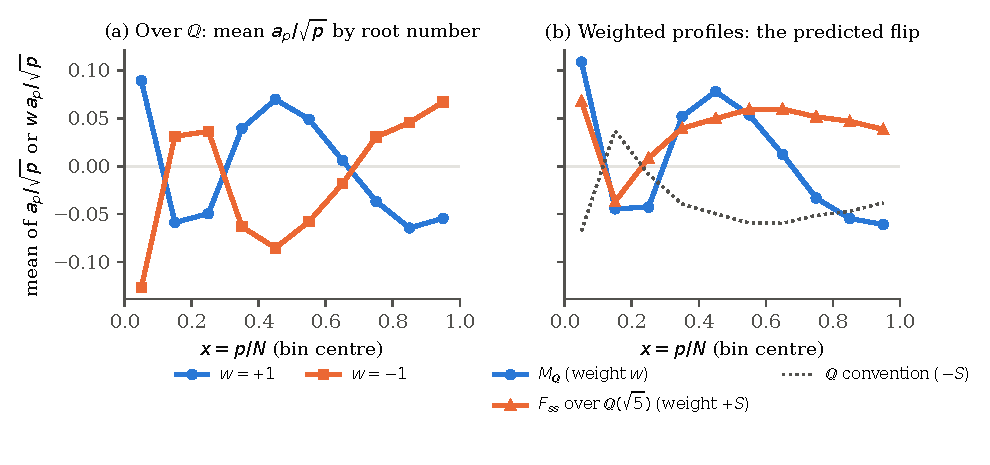
\includegraphics[width=\textwidth]{figures/fig_murmurations.pdf}
\caption{Part A. (a) Over $\Q$: mean of $a_p/\sqrt p$ for $w=+1$ and $w=-1$. (b) The weighted profile $M_\Q$ and, over $\Kfield$, the profile $F_{ss}$ weighted by $+S$; the dotted line is what the rule of $\Q$ ($-S$) would give.}\label{fig:murm}
\end{figure}

\begin{table}[ht]
\centering\small
\caption{Part A: binned profiles on the confirmatory ranges (bins labelled by their left end).}\label{tab:partA}
\setlength{\tabcolsep}{3.5pt}
\begin{tabular}{@{}lrrrrrrrrrr@{}}
\toprule
$x=p/N$ & $0.0$ & $0.1$ & $0.2$ & $0.3$ & $0.4$ & $0.5$ & $0.6$ & $0.7$ & $0.8$ & $0.9$\\
\midrule
$M_\Q$ & $.1087$ & $-.0445$ & $-.0427$ & $.0518$ & $.0778$ & $.0536$ & $.0123$ & $-.0333$ & $-.0546$ & $-.0609$\\
$F_{ss}$ & $.0677$ & $-.0370$ & $.0084$ & $.0395$ & $.0496$ & $.0593$ & $.0596$ & $.0515$ & $.0469$ & $.0384$\\
\bottomrule
\end{tabular}
\end{table}

\subsection{Part B: local signs and rank}
To remove the conductor as a confound, Part~B compares only classes that share a conductor, a kind of address that fixes their bad primes and exponents, so that classes at the same address differ only in their signs. Conductors below $300{,}000$ are for training, $300{,}000$ to $399{,}999$ for validation, and $400{,}000$ to $499{,}999$ for the single held-out test ($209{,}944$ classes). An experiment receives each class as its conductor and its list of bad primes with exponents and local signs, never $a_p$ or the curve, and returns a score for rank~$2$. The metric is the within-conductor AUC: over all pairs of a rank-$2$ and a rank-$0$ class with the same conductor, the fraction in which the rank-$2$ class scores higher. It has a simple reading. Pick a rank-$2$ curve and a rank-$0$ curve at the same address, show a rule only their signs, and ask it which is which; the AUC is the fraction of correct guesses, so $0.5$ is a coin flip and $1$ is perfect. Two hypotheses were fixed in advance, each to be tested one-sided at $p<0.01$:

\begin{hypothesis}[H$_{B1}$]
The number of split multiplicative primes (bad primes with $w_p=-1$ and exponent one) has within-conductor AUC above $0.5$ on the test conductors.
\end{hypothesis}

\begin{hypothesis}[H$_{B2}$]
The rule promoted by the laboratory has within-conductor AUC above $0.5$ on the test conductors.
\end{hypothesis}

\emph{The search.} The laboratory used $25$ of its $40$ validation evaluations and kept three changes, raising the validation score from $0.521$ to $0.539$. The largest and simplest was to count the $-1$ signs at primes $p\ge5$ and subtract those at $p=2$ and $3$: a $-1$ at a larger prime points towards rank~$2$, and one at $2$ or $3$ towards rank~$0$. The other two refined this count with a cautious table, learned on training conductors, of how often each pattern of local reduction types carries rank~$2$, distinguishing additive primes $p\ge5$ by $p\bmod 4$. Flexible models that looked good on validation failed on a separate slice of training data, and the Skeptic rejected two trials that met the numerical keep rule, one because it exploited the set of patterns present at a conductor and one because a placebo did as well.

\emph{The final rule.} The promoted rule starts from the size count above. It then describes each bad prime by its size, its reduction type (multiplicative or additive), for additive $p\ge5$ the residue $p\bmod4$, and its sign, and nudges the count by the log-odds of rank~$2$ observed in training for the same pattern, shrunk towards the count when the pattern is rare. By Rohrlich's formulas \cite{Rohrlich1993}, at an additive prime $p\ge5$ the local sign equals $(-1/p)$ except possibly for Kodaira types III, III$^*$, IV and IV$^*$, so the residue modulo $4$ lets the table distinguish these types from the generic ones. Figure~\ref{fig:loop} shows the course of the search.

\begin{figure}[ht]
\centering
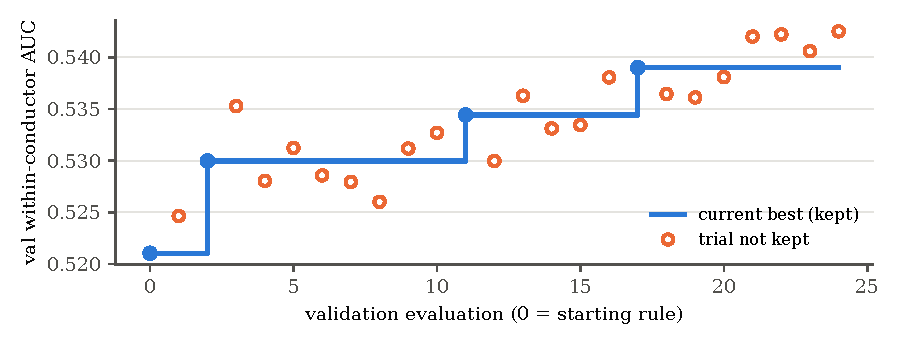
\includegraphics[width=0.82\textwidth]{figures/fig_loop.pdf}
\caption{Part B on the validation set. Each circle is one evaluation; the line is the current best, which moves only when the Skeptic approves a trial that meets the keep rule.}\label{fig:loop}
\end{figure}

\emph{Held-out results.} Table~\ref{tab:partB} and Figure~\ref{fig:partB} give the single final run, on about $210{,}000$ curves that no person or agent had examined before. Both hypotheses are supported, with permutation $p$-values at their floor of $1/2001$ and normal-approximation $p$-values far below one in a million. In the language of the guessing game, the rule fixed in advance is right $52\%$ of the time and the laboratory's rule $54\%$, while a rule allowed to see the solution counts $a_p$ is right $96\%$ of the time: almost all of the difference between the ranks lies elsewhere, but the signs carry a real trace. The laboratory's rule improves on the simple rule by $0.021$ (paired interval $[0.014,0.028]$), and its test score is slightly above its validation score. A positive control that may use $a_p$ at the good primes below $100$ shows the scale of a strong rank signal.

\begin{table}[ht]
\centering\small
\caption{Part B on the test conductors $400{,}000\le N<500{,}000$ (one run; $775{,}454$ pairs).}\label{tab:partB}
\begin{tabular}{@{}lcccc@{}}
\toprule
Score & AUC & 95\% interval & $z$ & verdict\\
\midrule
H$_{B1}$: split multiplicative count & $0.522$ & $[0.517,0.527]$ & $8.6$ & supported\\
H$_{B2}$: laboratory's rule & $0.543$ & $[0.536,0.550]$ & $15.1$ & supported\\
Positive control (uses $a_p$, $p<100$) & $0.964$ & $[0.962,0.965]$ & $160$ & \\
\bottomrule
\end{tabular}
\end{table}

\begin{figure}[ht]
\centering
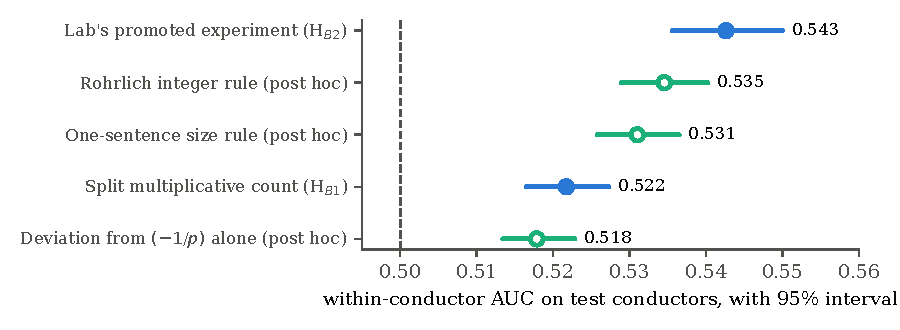
\includegraphics[width=0.88\textwidth]{figures/fig_partB_test.pdf}
\caption{Part B on the test conductors. Filled circles are the pre-registered hypotheses; open circles are rules suggested by the analysis and scored only after the final run (post hoc). The dashed line is $0.5$.}\label{fig:partB}
\end{figure}

\emph{Post hoc checks.} After the final run we scored, on the test conductors, simple rules suggested by the analysis but not named in advance. The one-sentence size rule scores $0.531$ and beats the pre-registered rule by $0.009$ (paired interval $[0.0035,0.015]$), in line with its validation gain. A rule that adds departures of the local sign from $(-1/p)$ at additive primes $p\ge5$, motivated by Rohrlich's formulas \cite{Rohrlich1993}, scores $0.535$, but its gain over the size rule is not significant (paired interval $[-0.0005,0.0076]$). The size effect is therefore robust, while the role of reduction type is only suggestive.

\emph{Replication.} At the author's direction, a separate Claude session that had built Artemis but took no part in the run rebuilt the promoted experiment from the laboratory's report, confirmed that its SHA-256 matches the promoted file, and ran the final test once on a fresh clone of the public repository. Every number in Table~\ref{tab:partB} and in Part~A was reproduced exactly.

% ======================================================================
\section{Discussion}\label{sec:discussion}

\emph{What is expected and what may be new.} Part~A confirms established theory; its contribution is a pre-registered demonstration of the archimedean sign inside murmurations over a real quadratic field, together with an unexplained difference in shape. We have not found a published study of murmurations over real quadratic fields, but our search was limited. The closest work is Martin's on the distribution of local root numbers of newforms and on murmurations weighted by partial root numbers \cite{Martin2023,Martin2024,Martin2025}. Part~B belongs to that line of work; what distinguishes it is the comparison of rank-$0$ and rank-$2$ curves within a single conductor. A specialist search of the literature should precede any claim of novelty.

\emph{Where the signal lives.} The sign vector does depend on rank, but weakly: almost all of the difference between rank~$0$ and rank~$2$ lies in the $a_p$ at good primes, and the local signs carry a small, statistically clear trace located mainly in the size of the bad prime. A natural hypothesis, not tested here, runs through the Birch--Swinnerton-Dyer formula: the reduction type at a bad prime fixes or nearly fixes its Tamagawa number, which enters the leading term where rank~$0$ and rank~$2$ curves differ. Adding Tamagawa numbers to the data would test this directly.

\emph{The scale over a number field.} The divergence of the profiles beyond $p/N\approx0.7$ suggests that the conductor norm alone is not the natural scale over $\Kfield$; a normalization involving the discriminant, or treating conjugate primes jointly, may align them.

\emph{Limits.} Ranks are as recorded in Cremona's tables and the LMFDB; the sample over $\Kfield$ is small and confined to norms below $5{,}000$; the effect in Part~B is small in absolute terms; and the validation set was used many times, so only the single test run is free of selection. The laboratory's ledger and archived trial code remained in its sandbox; its report, its promoted code and the replication are public.

\emph{What it means.} The paper does not prove a theorem or settle a famous problem. It offers a way of seeing a familiar fact, Euler's half turn as the common source of many signs, a confirmation of that view in real data, and one small new observation about how the signs of elliptic curves relate to their ranks, with a list of next steps.

\emph{AI laboratories.} The agents worked on their own, found a rule a mathematician can state in one sentence, and discarded clever models that did not hold up. But the most consequential event of the project was a leak in the data that a careless harness would have rewarded, caught only because a second agent was asked to attack the first one's work. The value of such a laboratory lies less in how clever its agents are than in the fixed rules, sealed data and independent checks that keep them honest.

% ======================================================================
\section{Research directions}\label{sec:directions}

\emph{R1. Murmurations as a probe of the archimedean sign [P].} Status after the first run: the flip over $\Kfield$ is confirmed, and local signs depend weakly on rank within a conductor. Next steps are a fresh pre-registered test of the reduction-type reading, a test of the Tamagawa mechanism, and Part~A over further totally real fields, where the predicted sign is $(-1)^d$.

\emph{R2. The odd/even wall [O].} Everything proved for $\GL_2$ over $\Q$ lies on the odd side, $\det\rho(c)=-1$. Over CM fields Galois representations exist in general \cite{HLTT2016,Scholze2015,Allen2023}, at the price of cohomology spread over several degrees \cite{Venkatesh2019}. Is the archimedean sign the degree-zero part of a graded archimedean datum that also governs that spread? A first step is to compare, for curves over $\Q$ base-changed to an imaginary quadratic field, the information lost in $w(E/K)=w(E)\,w(E\otimes\chi_K)$ with the derived action on the cohomology of the Bianchi group.

\emph{R3. Cubic Gauss sums [O].} For $n=2$ the real place cancels the finite Gauss-sum signs; for $n=3$ the complex place contributes nothing, and Patterson's bias, now a theorem under the generalized Riemann hypothesis \cite{DunnRadziwill2024}, is a secondary term. Can the bias constant be read as a contribution of the complex place to a Weil-index-type product formula for the cubic theta function \cite{KazhdanPatterson1984}? A first step is to compare it with the constant term of that theta function at the archimedean place.

\emph{R4. Theta characteristics [O].} Geometric Langlands requires a choice of square root of the canonical bundle, which carries an Arf parity \cite{Atiyah1971}. Does the now-proved equivalence \cite{GaitsgoryRaskin2024} change under this choice by a sign that is the geometric analogue of $i^k$? Curves of genus one, with three even and one odd theta characteristic, are the first test case.

\emph{R5. The prime $2$ [P].} The prime $2$ is the only one for which $-1$ is a $p$-power root of unity, and many exceptional phenomena at $2$ (including the ``twice a square'' case of Poonen and Stoll \cite{PoonenStoll1999}) may admit one formulation through the interaction of $-1\in\Q_2$ with complex conjugation, for instance by writing them as instances of Deligne's product formula for orthogonal local constants \cite{Deligne1976}.

\emph{R6. Sato--Tate groups as compact Weil groups [P].} For which motives is the Sato--Tate group the maximal compact subgroup of an archimedean-type Weil group, and what does its trace-zero component look like in higher dimension \cite{FKRS2012}?

\emph{R7. A catalogue of sign reciprocities [P].} The product formulas for local signs met above each have an archimedean term equal to $-1$ or its square root; we conjecture that all are $2$-torsion of the Brauer--Hasse--Noether sequence, so that a sign reciprocity not of this form would be new.

\emph{R8. The only closed-form archimedean sign [O].} Because $\mu(\R)=\{\pm1\}$, a ``higher Euler identity'' would have to live at finite places, a useful negative constraint on what to look for.

% ======================================================================
\section*{Numerical checks, code and data}
A Python script, included as an ancillary file and in the repository, verifies numerically the identities used in Section~\ref{sec:synthesis}; all $46$ checks pass (Table~\ref{tab:checks}).

\begin{table}[ht]
\centering\small
\caption{Numerical checks (mpmath at 40 digits; PARI/GP for elliptic curves).}\label{tab:checks}
\begin{tabular}{@{}lr@{}}
\toprule
Identity & checks\\
\midrule
$e^{i\pi}=-1$ and its square roots & 3\\
$\zeta(2k)/(2\pi i)^{2k}=-B_{2k}/2(2k)!$ for $k\le6$ & 6\\
Gauss-sum signs $g_p=i^{((p-1)/2)^2}\sqrt p$, first ten odd primes & 10\\
Weil index $\int_\R e^{i\pi x^2}dx=e^{i\pi/4}$ & 2\\
Landsberg--Schaar relation, seven pairs & 7\\
Transformation laws of $E_6$, $\Delta$, $\Delta E_6$; $E_6(i)=0$ & 4\\
$(-1)^{\mathrm{rank}}=-w_N=a_N$ for 11a1, 37a1, 43a1, 389a1, 5077a1 & 5\\
Dwork's $\theta(1)$ is a primitive $p$-th root of unity, $p=3,5,7$ & 3\\
$\Gamma_\R$ as a Gaussian integral; Fourier eigenvalues & 4\\
CM Sato--Tate law for $y^2=x^3-x$ and $y^2=x^3+1$, $p<10^5$ & 2\\
\bottomrule
\end{tabular}
\end{table}

The laboratory, the frozen harness and data of this program, the promoted experiment, the laboratory's report and the replication are public at \url{https://github.com/alessoh/artemis} on the branch \texttt{langlands-lab}.

\section*{Use of AI tools}
The Artemis software was written by Claude (Anthropic) as a coding agent under the author's direction, and an independent Claude agent audited it before the run. The experiment was carried out autonomously by the Artemis agents (Claude Opus~5.5 and Claude Haiku~4.5) under the pre-registered rules. The replication, the post hoc checks and the numerical checks were performed by a separate Claude session (Claude Opus~5.5) that took no part in the run and that also drafted this manuscript from the author's notes and the result files; a further Claude agent reviewed it as a referee. The author revised the manuscript and takes full responsibility for its content; no AI system is an author.

\section*{Acknowledgments}
Artemis was built for Challenge 03 of the 7th Global AI Hackathon. We thank John Cremona and the LMFDB collaboration for making their data public, and the developers of PARI/GP, Omnigent and Modal.

% Bibliography (generated by BibTeX from refs.bib, amsplain style)
\providecommand{\bysame}{\leavevmode\hbox to3em{\hrulefill}\thinspace}
\providecommand{\MR}{\relax\ifhmode\unskip\space\fi MR }
% \MRhref is called by the amsart/book/proc definition of \MR.
\providecommand{\MRhref}[2]{%
  \href{http://www.ams.org/mathscinet-getitem?mr=#1}{#2}
}
\providecommand{\href}[2]{#2}
\begin{thebibliography}{10}

\bibitem{Allen2023}
Patrick~B. Allen, Frank Calegari, Ana Caraiani, Toby Gee, David Helm, Bao~V.
  Le~Hung, James Newton, Peter Scholze, Richard Taylor, and Jack~A. Thorne,
  \emph{Potential automorphy over {CM} fields}, Ann. of Math. (2) \textbf{197}
  (2023), 897--1113.

\bibitem{GaitsgoryRaskin2024}
D.~Arinkin, D.~Beraldo, J.~Campbell, L.~Chen, J.~F{\ae}rgeman, D.~Gaitsgory,
  K.~Lin, S.~Raskin, and N.~Rozenblyum, \emph{Proof of the geometric
  {L}anglands conjecture {I}--{V}}, 2024, arXiv:2405.03599 and sequels.

\bibitem{Arthur2013}
James Arthur, \emph{The endoscopic classification of representations:
  Orthogonal and symplectic groups}, Amer. Math. Soc. Colloq. Publ., vol.~61,
  Amer. Math. Soc., 2013.

\bibitem{ArtinSchreier1927}
Emil Artin and Otto Schreier, \emph{Eine {K}ennzeichnung der reell
  abgeschlossenen {K}{\"o}rper}, Abh. Math. Sem. Univ. Hamburg \textbf{5}
  (1927), 225--231.

\bibitem{Atiyah1971}
Michael~F. Atiyah, \emph{Riemann surfaces and spin structures}, Ann. Sci.
  {\'E}cole Norm. Sup. (4) \textbf{4} (1971), 47--62.

\bibitem{BellaicheChenevier2011}
Jo{\"e}l Bella{\"\i}che and Ga{\"e}tan Chenevier, \emph{The sign of {G}alois
  representations attached to automorphic forms for unitary groups}, Compos.
  Math. \textbf{147} (2011), 1337--1352.

\bibitem{Brown2012}
Francis Brown, \emph{Mixed {T}ate motives over {$\mathbb Z$}}, Ann. of Math.
  (2) \textbf{175} (2012), 949--976.

\bibitem{Calegari2011}
Frank Calegari, \emph{Even {G}alois representations and the {F}ontaine--{M}azur
  conjecture}, Invent. Math. \textbf{185} (2011), 1--16.

\bibitem{Carlitz1935}
Leonard Carlitz, \emph{On certain functions connected with polynomials in a
  {G}alois field}, Duke Math. J. \textbf{1} (1935), 137--168.

\bibitem{Ecdata}
J.~E. Cremona, \emph{Elliptic curve data ({\tt ecdata})},
  \url{https://github.com/JohnCremona/ecdata}, commit 25cec5e.

\bibitem{Deligne1973}
Pierre Deligne, \emph{Les constantes des {\'e}quations fonctionnelles des
  fonctions {L}}, Modular Functions of One Variable {II}, Lecture Notes in
  Math., vol. 349, Springer, 1973, pp.~501--597.

\bibitem{Deligne1976}
\bysame, \emph{Les constantes locales de l'{\'e}quation fonctionnelle de la
  fonction {L} d'{A}rtin d'une repr{\'e}sentation orthogonale}, Invent. Math.
  \textbf{35} (1976), 299--316.

\bibitem{Deligne1979}
\bysame, \emph{Valeurs de fonctions {L} et p{\'e}riodes d'int{\'e}grales},
  Automorphic Forms, Representations and {L}-functions, Part 2, Proc. Sympos.
  Pure Math., vol.~33, Amer. Math. Soc., 1979, pp.~313--346.

\bibitem{DeligneGoncharov2005}
Pierre Deligne and Alexander~B. Goncharov, \emph{Groupes fondamentaux
  motiviques de {T}ate mixte}, Ann. Sci. {\'E}cole Norm. Sup. (4) \textbf{38}
  (2005), 1--56.

\bibitem{DokchitserDokchitser2010}
Tim Dokchitser and Vladimir Dokchitser, \emph{On the
  {B}irch--{S}winnerton-{D}yer quotients modulo squares}, Ann. of Math. (2)
  \textbf{172} (2010), 567--596.

\bibitem{DunnRadziwill2024}
Alexander Dunn and Maksym Radziwi{\l}{\l}, \emph{Bias in cubic {G}auss sums:
  {P}atterson's conjecture}, Ann. of Math. (2) \textbf{200} (2024).

\bibitem{Dwork1960}
Bernard Dwork, \emph{On the rationality of the zeta function of an algebraic
  variety}, Amer. J. Math. \textbf{82} (1960), 631--648.

\bibitem{FKRS2012}
Francesc Fit{\'e}, Kiran~S. Kedlaya, V{\'\i}ctor Rotger, and Andrew~V.
  Sutherland, \emph{Sato--{T}ate distributions and {G}alois endomorphism
  modules in genus 2}, Compos. Math. \textbf{148} (2012), 1390--1442.

\bibitem{Fontaine1994}
Jean-Marc Fontaine, \emph{Le corps des p{\'e}riodes $p$-adiques},
  Ast{\'e}risque \textbf{223} (1994), 59--111.

\bibitem{FreitasLeHungSiksek2015}
Nuno Freitas, Bao~V. Le~Hung, and Samir Siksek, \emph{Elliptic curves over real
  quadratic fields are modular}, Invent. Math. \textbf{201} (2015), 159--206.

\bibitem{Gauss1811}
Carl~Friedrich Gauss, \emph{Summatio quarumdam serierum singularium},
  Commentationes Societatis Regiae Scientiarum Gottingensis Recentiores
  \textbf{1} (1811).

\bibitem{GrossZagier1986}
Benedict~H. Gross and Don~B. Zagier, \emph{Heegner points and derivatives of
  {L}-series}, Invent. Math. \textbf{84} (1986), 225--320.

\bibitem{HLTT2016}
Michael Harris, Kai-Wen Lan, Richard Taylor, and Jack Thorne, \emph{On the
  rigid cohomology of certain {S}himura varieties}, Res. Math. Sci. \textbf{3}
  (2016), Paper No. 37.

\bibitem{HLOP2022}
Yang-Hui He, Kyu-Hwan Lee, Thomas Oliver, and Alexey Pozdnyakov,
  \emph{Murmurations of elliptic curves}, 2022, arXiv:2204.10140; Experiment.
  Math. (2024), doi:10.1080/10586458.2024.2382361.

\bibitem{HeathBrownPatterson1979}
D.~R. Heath-Brown and S.~J. Patterson, \emph{The distribution of {K}ummer sums
  at prime arguments}, J. Reine Angew. Math. \textbf{310} (1979), 111--130.

\bibitem{Isaacson2023}
Walter Isaacson, \emph{Elon {M}usk}, Simon \& Schuster, New York, 2023.

\bibitem{KapustinWitten2007}
Anton Kapustin and Edward Witten, \emph{Electric-magnetic duality and the
  geometric {L}anglands program}, Commun. Number Theory Phys. \textbf{1}
  (2007), 1--236.

\bibitem{Karpathy2026}
Andrej Karpathy, \emph{autoresearch}, Software repository,
  \url{https://github.com/karpathy/autoresearch}.

\bibitem{KazhdanPatterson1984}
D.~A. Kazhdan and S.~J. Patterson, \emph{Metaplectic forms}, Inst. Hautes
  {\'E}tudes Sci. Publ. Math. \textbf{59} (1984), 35--142.

\bibitem{KhareWintenberger2009}
Chandrashekhar Khare and Jean-Pierre Wintenberger, \emph{Serre's modularity
  conjecture ({I})}, Invent. Math. \textbf{178} (2009), 485--504.

\bibitem{Kottwitz1983}
Robert~E. Kottwitz, \emph{Sign changes in harmonic analysis on reductive
  groups}, Trans. Amer. Math. Soc. \textbf{278} (1983), 289--297.

\bibitem{LanglandsProblems1970}
Robert~P. Langlands, \emph{Problems in the theory of automorphic forms},
  Lectures in Modern Analysis and Applications {III}, Lecture Notes in Math.,
  vol. 170, Springer, 1970, pp.~18--61.

\bibitem{Langlands1973}
\bysame, \emph{On the classification of irreducible representations of real
  algebraic groups}, Representation Theory and Harmonic Analysis on Semisimple
  {L}ie Groups, Math. Surveys Monogr., vol.~31, Amer. Math. Soc., 1989,
  Preprint 1973, pp.~101--170.

\bibitem{Martin2023}
Kimball Martin, \emph{Root number bias for newforms}, Proc. Amer. Math. Soc.
  \textbf{151} (2023), 3721--3736, arXiv:2207.08121.

\bibitem{Martin2024}
\bysame, \emph{Distribution of local signs of modular forms and murmurations of
  {F}ourier coefficients}, 2024, arXiv:2409.02338; Mathematika (2025).

\bibitem{Martin2025}
\bysame, \emph{Variations on murmurations}, 2025, arXiv:2505.01093.

\bibitem{Omnigent}
{Omnigent contributors}, \emph{Omnigent}, Software repository,
  \url{https://github.com/omnigent-ai/omnigent}.

\bibitem{PoonenStoll1999}
Bjorn Poonen and Michael Stoll, \emph{The {C}assels--{T}ate pairing on
  polarized abelian varieties}, Ann. of Math. (2) \textbf{150} (1999),
  1109--1149.

\bibitem{Rohrlich1993}
David~E. Rohrlich, \emph{Variation of the root number in families of elliptic
  curves}, Compos. Math. \textbf{87} (1993), 119--151.

\bibitem{Scholze2015}
Peter Scholze, \emph{On torsion in the cohomology of locally symmetric
  varieties}, Ann. of Math. (2) \textbf{182} (2015), 945--1066.

\bibitem{Tate1950}
John Tate, \emph{Fourier analysis in number fields and {H}ecke's
  zeta-functions}, Algebraic Number Theory (J.~W.~S. Cassels and
  A.~Fr{\"o}hlich, eds.), Academic Press, 1967, Thesis, Princeton, 1950,
  pp.~305--347.

\bibitem{Tate1979}
\bysame, \emph{Number theoretic background}, Automorphic Forms, Representations
  and {L}-functions, Part 2, Proc. Sympos. Pure Math., vol.~33, Amer. Math.
  Soc., 1979, pp.~3--26.

\bibitem{LMFDB}
{The LMFDB Collaboration}, \emph{The {L}-functions and modular forms database},
  \url{https://www.lmfdb.org}, elliptic curves over 2.2.5.1, accessed 8 October
  2026.

\bibitem{PARI}
{The PARI Group}, \emph{{PARI/GP} version 2.17.2},
  \url{https://pari.math.u-bordeaux.fr}.

\bibitem{Venkatesh2019}
Akshay Venkatesh, \emph{Derived {H}ecke algebra and cohomology of arithmetic
  groups}, Forum Math. Pi \textbf{7} (2019), e7.

\bibitem{Weil1964}
Andr{\'e} Weil, \emph{Sur certains groupes d'op{\'e}rateurs unitaires}, Acta
  Math. \textbf{111} (1964), 143--211.

\bibitem{Zubrilina2023}
Nina Zubrilina, \emph{Murmurations}, 2023, arXiv:2310.07681.

\end{thebibliography}


\end{document}
